\section{Results}\label{sec:results}

\paragraph{T1: representation.} Every instance is one connected component, so every junction can be supplied by some source. BFS on the matrix is 8.3 (NYT) to 22.6 (PES) times slower than on the list, because each visited vertex scans a full row. Memory is close at this size: a list entry is a Python tuple plus a float (about 120 bytes per pipe end) against 8 bytes per matrix cell, so the list is slightly larger on NYT (5.7 against 4.7 KiB), but the matrix grows quadratically and doubles the list on PES (44.6 against 23.3 KiB). The matrix only wins the pipe-existence query (67 against about 135 ns), so the list is the working representation and the matrix is used only for all-pairs tables.

\paragraph{T2: pipe lengths.} Table~\ref{tab:lengths} gives the length statistics. Length and capacity are distinct attributes (correlation $-0.65$ to $+0.13$). The FOS mesh keeps every pair within 1.75 times its straight-line distance, while NYT and HAN reach 4.73 and 3.32. PES is extreme: nodes 19 and 39 are 147 units apart but 4,146 by pipe, because PES is two dense clusters joined by few pipes. On average network distances are 19\% (FOS) to 83\% (PES) longer than straight lines, which is why T3 and T4 use $d_G$. The hash index answers a length query in 0.09\,\textmu s against 6.5\,\textmu s for a scan, and the sorted array finds the 9 PES pipes longer than 1,000 with 7 comparisons instead of 98.

\begin{table}[H]
\centering\small
\caption{Pipe lengths (coordinate units) and circuity $d_G/\lVert p_u-p_v\rVert$ over all node pairs.}\label{tab:lengths}
\begin{tabular}{lrrlrlrrrr}
\toprule
\tablebody{lengths}
\bottomrule
\end{tabular}
\end{table}

\paragraph{T3: sectors.} Figure~\ref{fig:freshness} shows the sectors (sizes in Table~\ref{tab:chain}). The pipes to close are 2--3, 11--9 and 20--16 in NYT; 7--8 and 14--15 in HAN; 18--19 and 19--20 in PES; and eight in the FOS mesh: 3--4, 28--9, 11--19, 27--16, 11--26, 16--29, 26--27 and 28--29. HAN's sectors are the most unequal (7 against 25 nodes) because source 13 sits behind a single 1,683-unit pipe at the network's edge. Multi-source Dijkstra used exactly half the heap operations of the repeated version (76 against 155 pops on PES).

\begin{figure}[H]
    \centering
    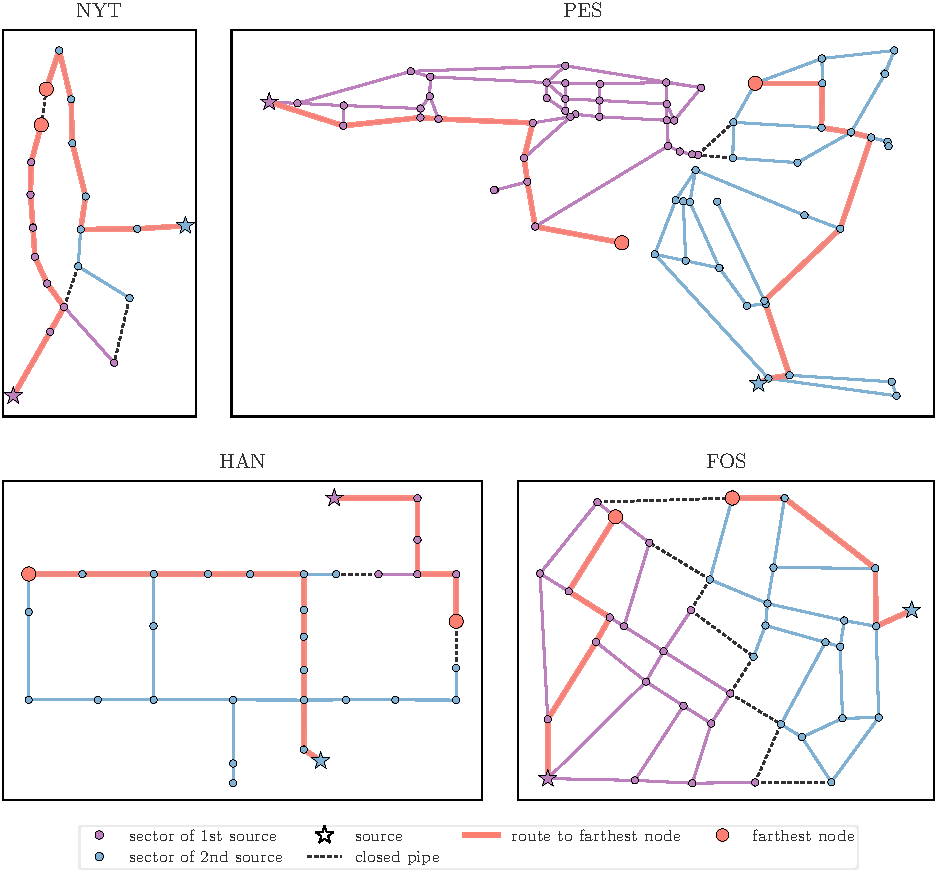
\includegraphics[width=0.92\textwidth]{freshness.pdf}
    \caption{T3 and T4. Sectors from multi-source Dijkstra (colour), closed pipes (dashed) and the shortest route from each source to the node of its sector that receives the oldest water.}
    \label{fig:freshness}
\end{figure}

\paragraph{T4: freshness.} Table~\ref{tab:chain} gives each sector's farthest node and distance; routes are drawn in Figure~\ref{fig:freshness} and listed in \texttt{04\_freshness}. Four of the eight (NYT 3 and 2, HAN 8, FOS 3) sit at a closed pipe, where the two supply areas meet; the others lie at the far end of their sector. Column ``Before'' divides the source's farthest distance in the open network by $d_G(s,t_s)$: sectorization reduces the worst water age a source is responsible for by 1.49 to 2.25 times in FOS and PES and by 2.75 times for HAN source 13; HAN source 1 is unaffected. Per node nothing changes, since closing $C$ leaves every distance to the node's own source intact.

\begin{table}[H]
\centering\small
\caption{Results chained per sector: size (T3), farthest node and distance (T4), maximum flow, capacity of the T4 route alone and minimum cut (T5).}\label{tab:chain}
\begin{tabular}{lrrrrrrrp{3.3cm}}
\toprule
\tablebody{chain}
\bottomrule
\end{tabular}
\end{table}

\paragraph{T5: maximum flow.} In six of the eight sectors the minimum cut is the single pipe at a leaf source (NYT, HAN, PES source 7) or leaf sink (PES 10), so the rest of the sector does not affect throughput. Comparing with the T4 route shows the difference between the two problems: PES source 1's shortest route carries only 101, but a second route into node 11 lets 151 reach node 10, and in the FOS mesh three disjoint bottleneck pipes carry 55 against 19 on the shortest route, and 58.8 against 17 in the other sector (Figure~\ref{fig:flows}). Making the cut pipes unlimited shows how capacity constrains the flow: the gain is nil in HAN, where every route is a chain of 16-capacity pipes, and reaches 3.6 times for FOS source 37 (58.8 to 211). Edmonds-Karp and Dinic always agree, with at most 4 augmenting paths.

\begin{figure}[H]
    \centering
    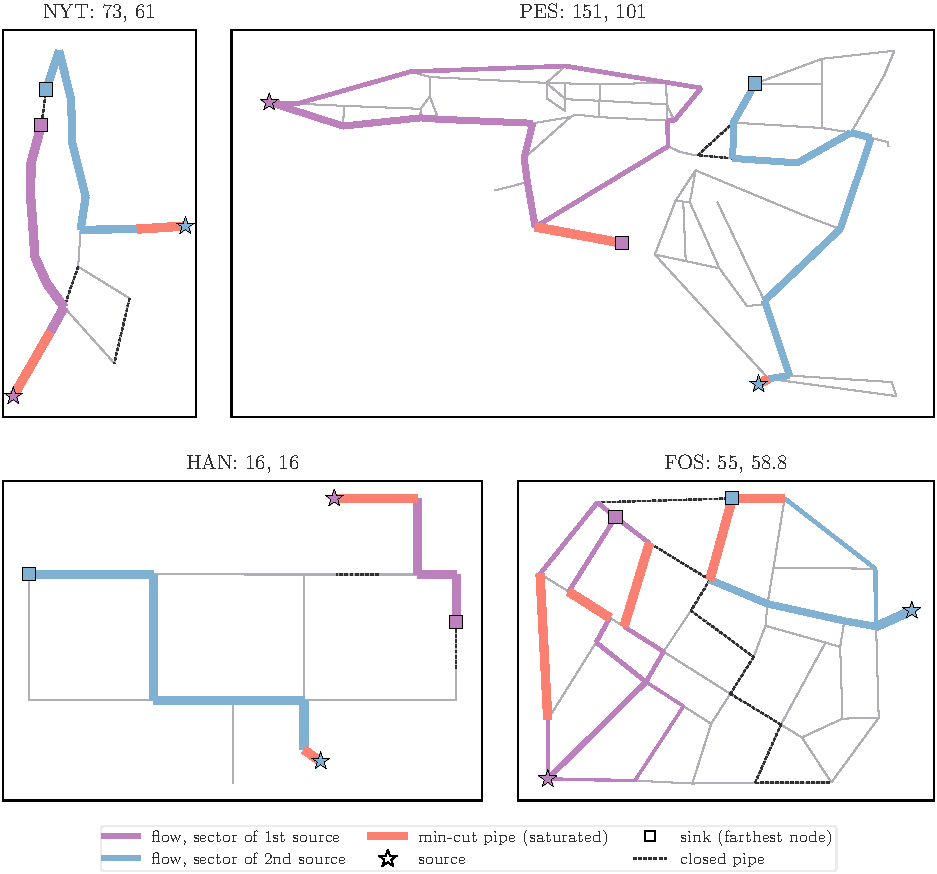
\includegraphics[width=\textwidth]{flows.pdf}
    \caption{T5 on the two meshed instances. Pipe width is proportional to flow; saturated minimum-cut pipes are highlighted. Titles give each sector's maximum flow.}
    \label{fig:flows}
\end{figure}

\paragraph{T6: sampling routes.} Table~\ref{tab:routes} compares the methods. NYT is solved exactly: the optimal walk has length 7,072 over 24 pipe traversals and walks both source branches there and back (Figure~\ref{fig:routes}a). For HAN, FOS and PES branch and bound does not finish within 60\,s, so their routes are 2-opt local optima, approximate and not certified: the MST bound is weak, especially on the near-tree HAN, where a walk traverses most pipes twice but the MST counts them once. On office-nearest subsets of $k=4,6,\dots$ nodes, solved exactly up to $k=18$ to 24, nearest neighbour is on average 15.9\% above the optimum (worst 37.8\%) and 2-opt 1.8\% (worst 15.8\%), optimal in 31 of 39 subsets (Figure~\ref{fig:routes}c).

\begin{table}[H]
\centering\small
\caption{Sampling routes. 2-opt gap: relative to the optimum when proven, otherwise an upper bound relative to the root lower bound. Walk pipes: pipe traversals of the expanded route.}\label{tab:routes}
\begin{tabular}{lrrrrlrrr}
\toprule
\tablebody{routes}
\bottomrule
\end{tabular}
\end{table}

\begin{figure}[H]
    \centering
    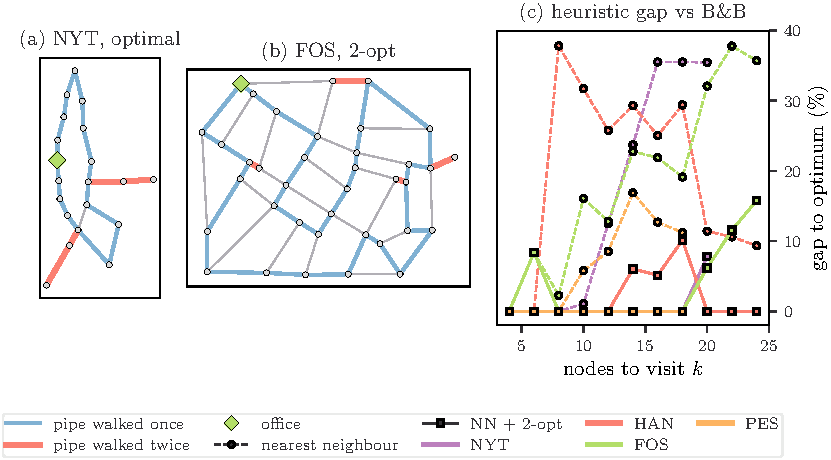
\includegraphics[width=\textwidth]{routes.pdf}
    \caption{T6. (a) Optimal NYT walk (7,072) and (b) best FOS walk found (30,424) from the office; pipes walked twice are highlighted. (c) Gap of nearest neighbour (dashed) and NN + 2-opt (solid) to the branch-and-bound optimum on office-nearest subsets.}
    \label{fig:routes}
\end{figure}

\paragraph{T7: expansion.} Table~\ref{tab:expansion} lists the insertions (Figure~\ref{fig:expansion}). The FOS point $(7071,9055)$ becomes node 38 linked to node 17, the connection drawn in the challenge slides. No new node is closest to an earlier new node, so insertion order does not matter here. On 2,000 random queries the 2-d tree evaluated on average 6.7 of 18 candidates on NYT and 11.0 of 69 on PES. Each insertion writes three list entries, whereas the matrix copies the whole table (10,225 cells for the two PES insertions).

\begin{table}[H]
\centering\small
\caption{New nodes, their nearest non-source node and the distance evaluations of each search.}\label{tab:expansion}
\setlength{\tabcolsep}{4pt}
\begin{tabular}{lrlrrrrr}
\toprule
\tablebody{expansion}
\bottomrule
\end{tabular}
\end{table}

\begin{figure}[H]
    \centering
    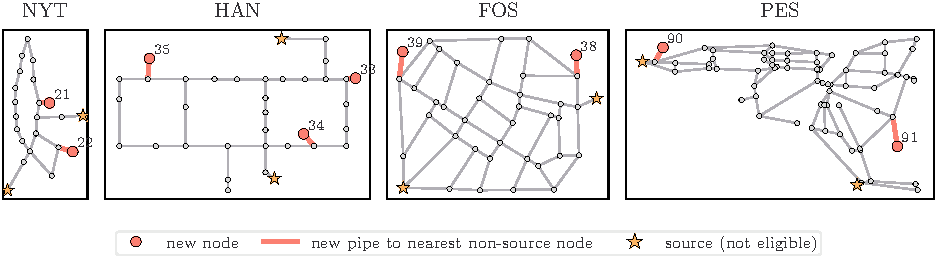
\includegraphics[width=\textwidth]{expansion.pdf}
    \caption{T7. Expanded networks: each new node is linked to its nearest non-source node.}
    \label{fig:expansion}
\end{figure}
